\section{API}
\label{section:api}

Ένα ακόμα πολύ σημαντικό συστατικό του διαδικτύου αποτελούν οι Διεπαφές Εφαρμογών Προγραμμάτων (Application Programming Interfaces - APIs).
Πρόκειται για το σύνολο των ορισμών, κανόνων και πρωτοκόλλων για τη δημιουργία και ενσωμάτωση μίας
εφαρμογής. Ουσιαστικά λειτουργεί ως το συμβόλαιο μεταξύ ενός συστήματος παροχής υπηρεσίας και του
χρήστη του συστήματος αυτού, καθορίζοντας την απαραίτητη πληροφορία που απαιτεί για να λειουργήσει σωστά
ο server αλλά και αντίστροφά, καθορίζοντας την απαραίτητη πληροφορία που απαιτεί ο client στην απάντηση
που θα του επιστραφεί.

Είναι εμφανές λοιπόν ότι σε κάθε περίπτωση, αν θέλει κανείς να αλληλεπιδράσει με κάποιο σύστημα
είτε για να αντλήσει πληροφορία, είτε για να στείλει πληροφορία (αποθήκευση ή τροποποίηση ήδη υπάρχουσας)
θα πρέπει να υπάρχουν κανόνες που ορίζουν και καθιστούν πιο εύκολη και απλή την επικοινωνία αυτή.

H έννοια του api δεν περιορίζεται φυσικά μόνο στο πλαίσιο του διαδικτύου, αλλά σε όλων των ειδών
εφαρμογές που υπάρχει επικοινωνία ενός κεντρικού σημείου (server) με κάποιον χρήστη (client) που θέλει να
κάνει χρήση των υπηρεσιών που αυτό προσφέρει.

Όσων αφορά τη διαθεσιμότητα και ασφάλεια των API, μπορούμε να διακρίνουμε τις εξής κατηγορίες:

\begin{itemize}
	\item \textbf{Ανοιχτά (Open):} Σε αυτού του τύπου διεπαφών λογισμικού, έχει ελεύθερη πρόσβαση καθένας,
		χωρίς να απαιτείται κάποια παραπάνω πληροφορία που αφορά την αυθεντικοποίηση ή ταυροποίηση του χρήστη.
		Επειδή ακριβώς η πληροφορία που παρέχεται (ανοιχτά) έιναι τεράστια, χρησιμοποιούνται πολύ
		συχνά σε έρευνες, όπως αυτή \cite{open_restful_api_analysis} που αξιοποιεί ελεύθερα προσβάσιμα
		πόρους για να αναλύσει τα πιο διαδεδομένα APIs. 
	\item \textbf{Δημόσια (Public):} Μοιάζουν πολύ με τα \textbf{Ανοιχτού Τύπου API}, με τη μόνη διαφορά, τον περιορισμό
		πρόσβασης σε ορισμένα σημεία που απαιτούν κλειδιά προκειμένουν να γίνει σε αντίθεση με πριν αυθεντικοποίηση και ταυτοποίηση. 
	\item \textbf{Ιδιωτικά (Private):} Αφορούν διεπαφές λογισμικού που αναπτύσσονται και χρησιμοποιούνται μόνο εντός ενός κλειστού
		πλαισίου, όπως θα μπορούσε να είναι μία επιχείρηση ή κάποιο πανεπιστήμιο που παρέχει ορισμένες υπηρεσίες μόνο εντός του χώρου του.
		Πολλές φορές στη βιβλιογραφία αναφέρονται και ως \textbf{Εσωτερικά (Internal APIs)}
	\item \textbf{Εταιρικά (Partner):} Είναι περιορισμένα στο πλήθος χρηστών που έχουν πρόσβαση σε αυτό. Χρησιμοποιούνται
		για επικοινωνία μεταξύ συστημάτων εταιριών/επιχειρήσεων για την ανάπτυξη και αξιοποίηση εφαρμογών και υπηρεσιών.
		Συνήθως η ασφάλεια σε όλες αυτές τις αλληλεπιδράσεις είναι αρκετά πιο αυστηρή.
	\item \textbf{Σύνθετα (Composite):} Συνδυάζουν περισσότερα από ένα API αιτημάτων σε ένα, κάνοντας έτσι 
		την επικοινωνία πιο αποδοτική (κερδίζοντας χρόνο από πολλά διαδοχικά API).
\end{itemize}

Αξίζει να σημειωθεί σε αυτό το σημείο ότι ο τρόπος δημιουργίας, η δομή καθώς και τα πρωτόκολλα που χρησιμοποιούν τα διαφόρα APIs που υπάρχουν στο διαδίκτυο
δεν είναι πάντα κοινά. Yπάρχουν κάποιες γνωστές αρχιτεκτονικές και πρωτόκολλα όπως θα δούμε και στη συνέχεια, που πέρα από τη δομή
των συστημάτων παρέχουν και κανόνες "Καλύτερων Πρακτικών" (Best Practices). Οι πιο γνωστές αριχτεκτόνικές
παρατίθενται στη συνέχεια:

\begin{itemize}
	\item \textbf{SOAP (Simple Object Access Protocol):} Χρησιμοποιούνταν ευρέως στο παρελθόν πριν την εμφάνιση του REST.
		Η επικοινωνία μεταξύ server και client επιτυγχάνεται με την αποστολή αρχείων XML.
	\item \textbf{RPC (Remote Procedure Call):} Αποτελεί πρωτόλλο επικοινωνίας που επιτρέπει σε ένα σύστημα (client) να καλεί διαδικασίες (procedures)
		ή συναρτήσεις σε ένα άλλο σύστημα (server) είτε αυτά είναι στο ίδιο δίκτυο, είτε απομακρυσμένα. Σκοπός είναι να
		κάνει τα δύο συστήματα να επικοινωνούν σαν να βρίσκονται στο ίδιο υπολογιστικό σύστημα. Επιγραμματικά η διαδικασία
		επικοινωνίας δύο συστημάτων ξεκινάει με ένα αίτημα στον server να εκτελέσει κάποια συγκεκριμένη λειτουργία, παρέχοντας
		ορίσματα που ίσως χρειαστούν για αυτό. Ο server τέλος επιστρέφει την απάντηση της παραπάνω διαδικασίας στον client. Σήμερα το πρωτόκολλο αυτό
		χρησιμοποιείται σε διάφορες εφαρμογές και αναπτύσσονται μάλιστα συνεχώς, σύχρονες τεχνολογίες που πατώντας πάνω στη βασική λειτουργία
		του πρωτοκόλλου κάνουν περαιτέρω βελτιστοποιήσεις (gRPC).
	\item \textbf{REST (Representational State Transfer)}: Η πιο διαδεδομένη μορφή API στο διαδίκτυο. Η λειτουργία του είναι απλή. Η χρήστης στέλνει αίτημα σε έναν
		απομακρυσμένο σύστημα (server). Το σύστημα αντιδράει και βάσει των δεδομένων που του στέλνει ο χρήστης, τρέχει διαδικασίες ώστε να παράξει το
		επιθυμητό αποτέλεσμα, το οποίο τέλος το αποστέλει στον client.
	\item \textbf{Websocket}: Αποτελεί πρωτόκολλο που επιτρέπει την αμφίδρομη επικοινωνία μεταξύ client και server. Σε αντίθεση με το REST API, που κάθε φορά
		που γίνεται ένα αίτημα στον server πρέπει να αποστέλλονται οι κατάλληλοι headers και να γίνεται η κατάλληλη σύνδεση μεταξύ των δύο συστημάτων, με τη χρήση των websockets
		η σύνδεση αυτή εκτελείται μόνο μία φορά στο αρχικό αίτημα που αποστέλλεται. Αξίζει να σημειωθεί ακόμα ότι θεωρείται ιδανικό για εφαρμογές που απαιτούν άμεση ενημέρωση \cite{websockets} (real-time-applications)
		τόσo για τον προαναφερθέντα λόγο, βάσει του οποίου μειώνεται δραστικά ο χρόνος επικοινωνίας μεταξύ των εμπλεκόμενων, όσο και για το γεγονός ότι
		μηνύματα μπορούν να σταλούν και από τη μεριά του client προς τον server αλλά και το ανάποδο (server σε client) χωρίς να χρειάζεται να γίνει κάποιο αίτημα πρώτα.
\end{itemize}

\subsection{RESTful API}
\label{subsec:rest_api}

Πρόκειται για ένα τύπο αρχιτεκτονικής λογισμικού για APIs, που αποτελείται από κατευθυντήριες γραμμές και βέλτιστες πρακτικές για τη δημιουργία επεκτάσιμων εφαρμογών στο διαδίκτυο.
Πρωτάθηκε το 2000, από τον Thomas Fielding \cite{rest_proposal} σαν ένας τρόπος για να κατευθύνει την ανάπτυξη εφαρμογών 
προκειμένου να υπάρχει ένα κοινός τρόπος "γραφής" ώστε να υπάρξη εξέλιξη στον τομέα αυτό ακόμα πιο γρήγορα και οργανωμένα.  
Το δομικό συστατικό του είναι το πρωτόκολλο HTTP που χρησιμοποιεί για να πραγματοποιεί κλήσεις μεταξύ συστημάτων.

Όπως προαναφέρθηκε ο τρόπος λειτουργίας στην απλούστερη έκδοσή του ξεκινάει με ένα αίτημα κάποιου χρήστη
σε ένα σύστημα της επιλογής του, παρέχοντας την απαραίτητη πληροφορία προκειμένου ο server να μπορέσει να αναταποκριθεί επιτυχώς.
Έπειτα, και αφού το σύστημα διεκπεραιώσει όλες τις εσωτερικές λειτουργίες του, απαντά μεταφέροντας πίσω στον χρήστη
την επιθυμητή πληροφορία και ενημερώνοντας τον σχετικά με την κατάσταση του αιτήματος του (σε περίπτωση που κάτι πήγε λάθος ο χρήστης
θα πρέπει να ενημερώνεται αναλόγως).

Ο βασικός τρόπος αλληλεπίδρασης με τους πόρους του συστήματος θα πρέπει να γίνεται
μέσα από τις τέσσερις βασικές μεθόδους του HTTP (\textbf{GET, POST, PUT, DELETE}), χωρίς αυτό να απαγορεύει
τη χρήση των υπόλοιπων. Κάθε σύστημα θα πρέπει τυπικά να υποστηρίζει CRUD λειτουργίες (Create, Read, Update, Delete)

Για να χαρακτηριστεί ένα API ώς RESTful θα πρέπει να ικανοποιεί τα παρακάτω, ενώ
στο \autoref{fig:rest_principles} μπορούμε να τα δούμε σε ένα γενικότερο πλαίσιο:

\begin{itemize}
	\item \textbf{Client-Server:} Τα δύο αυτά υπολογιστικά συστήματα θα πρέπει να είναι ανεξάρτητα.
		Πρακτικά αυτό σημαίνει ότι ο client θα ασχοληθεί αποκλειστικά και μόνο με το κομμάτι παρουσιάσης της πληροφορίας, που του παρέχει ο server,
		στον χρήστη μέσα από διεπαφές γραφικού χαρακτήρα, ενώ ο server θα εκτελεί μόνο λειτουργίες που αφορούν την δημιουργία, τροποποίηση και διαγραφή των πόρων του
		συστήματος. Με αυτό τον διαχωρισμό πλέον o client είναι πιο ελαφρής, καθώς διαχειρίζεται μόνο πληροφορία που του έρχεται έτοιμη από το σύστημα,
		και ο server μπορεί να κάνει πιο εύκολα scaling.
	\item \textbf{Cacheable:} ο client θα πρέπει να αποθηκεύει προσωρινά (cache) τις
		απαντήσεις που λαμβάνει από τον server για την αποφυγή συνεχών επαναλαμβανόμενων αιτημάτων, βελτιώνοντας
		έτσι την απόδοση του συστήματος.
	\item \textbf{Stateless:} Η πληροφορία της κατάστασης του συστήματος δεν θα πρέπει να αποθηκεύεται
		αλλά κάθε αίτημα θα πρέπει να περιέχει την απαραίτητη πληροφορία για να εκτελεστεί από τη μεριά του server.
		Η πληροφορία αυτή μπορεί να αποτελεί μέρος του ίδου του url, του body, των headers ή του query.
	\item \textbf{Πολυεπίπεδο Σύστημα (Layered System):} Τα υπολογιστικά συστήματα που συμμετέχουν στη διαδικασία αυτή δεν
		θα πρέπει να γνωρίζουν αν είναι άμεσα συνδεδεμένα μεταξύ τους ή υπάρχουν ενδιάμεσοι κόμβοι που παρεμβάλλονται.
		Το σύστημα θα πρέπει να λειτουργεί δίχως να έχει επίγνωση των γειτόνων του, περιμένοντας απλά την κατάλληλη πληροφορία για να
		λειτουργήσει, τόσο από τη μεριά του server όσο και από τη μεριά του client.
\end{itemize}

\begin{figure}[!ht]
	\centering
	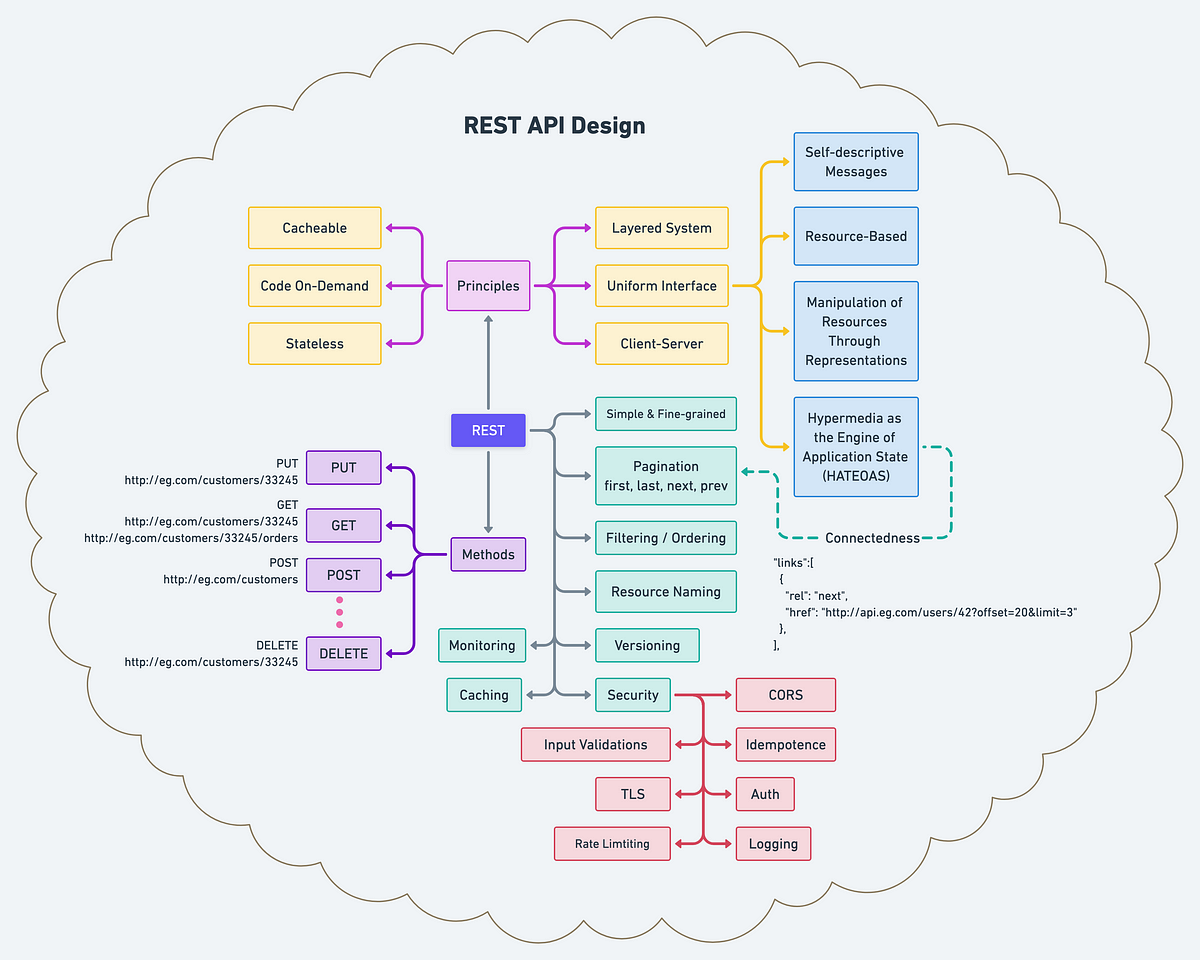
\includegraphics[width=0.8\textwidth]{./images/chapter2/rest_principles.png}
	\caption[Αρχές και Καλές Πρακτικές Σχεδίασης REST API]{Αρχές και Καλές Πρακτικές Σχεδίασης REST API}
	\label{fig:rest_principles}
\end{figure}